%---Preamble---
\documentclass[12pt,a4paper,titlepage]{article}
\usepackage[utf8]{inputenc}
\usepackage[T1]{fontenc}
\usepackage{lmodern}
\usepackage[ngerman]{babel}
\usepackage{longtable}
\usepackage{booktabs}
\usepackage{graphicx}
\usepackage{float}
\usepackage{xcolor}
\definecolor{black}{gray}{0} % 10% gray 
\usepackage[colorlinks=true,linkcolor=black,citecolor=black]{hyperref}
\usepackage[normalem]{ulem}
\usepackage{listings}
\usepackage{hyperref}
\usepackage{mathtools}
\usepackage{algorithm}
\usepackage{algorithmic}
\usepackage{subfigure}

\parindent 0pt
\parskip 8pt

%---Funktionen--
%Funktionen für Latex-Dokumente

\usepackage{ifthen}

%figure with citation
%\fig[width]{file}{label}{caption}{cite}
\newcommand{\fig}[5][1]{
\begin{figure}[!htbp]
\begin{center}
\includegraphics[width=#1\linewidth]{#2}
\caption[#4]{#4\ifthenelse{\equal{#5}{}}{}{~\cite{#5}}}
\label{#3}
\end{center}
\end{figure}
}

%Trademark Copyright
\newcommand{\tcopy}[0]{
\textsuperscript{\textcopyright}
}

\newcommand{\figref}[1]{
Abbildung~\ref{#1}
}

\newcommand{\secref}[1]{
Abschnitt~\ref{#1}
}

\newcommand{\enlargepage}[0]{
\enlargethispage{\baselineskip}
}

\usepackage{xspace}
\newcommand{\boidbot}[0]{BoidBot $A_{2}R$\xspace}

\begin{document}

%%%%%%%%%%%%%%%%%%%%%%%%%%%%
% Titelseite
%%%%%%%%%%%%%%%%%%%%%%%%%%%%
\begin{titlepage}
\begin{center}

{\large Autonome Systeme\\[0.1cm]
Hochschule für Technik und Wirtschaft\\[0.1cm]
SS2011}\\[1.5cm]
\rule{\linewidth}{0.3mm}\\[1.5cm]
{\huge BoidBot $A_{2}R$}\\[1cm]
{\LARGE --- Dokumentation ---}\\[1.5cm]
\rule{\linewidth}{0.3mm}\\[1.5cm]
{\large \today}\\[1cm]
\textbf{Andreas Bilke, B.\,Sc.}\\(andreas.bilke@student.htw-berlin.de)\\[0.3cm]
\textbf{Andreas Günther, B.\,Sc.}\\(andreas.guenther@student.htw-berlin.de)\\[3cm]
\end{center}
\end{titlepage}
\newpage

%%%%%%%%%%%%%%%%%%%%%%%%%%%%
% Inhaltsverzeichnis
%%%%%%%%%%%%%%%%%%%%%%%%%%%%
\pagenumbering{roman}
\tableofcontents
\newpage
\pagenumbering{arabic}

%%%%%%%%%%%%%%%%%%%%%%%%%%%%
% Inhalt
%%%%%%%%%%%%%%%%%%%%%%%%%%%%

\section{Aufgabenstellung}

Ziel der Vorlesung Autonome Systeme war es einen Roboter zu entwickeln, der eine frei gewählte Aufgabe lösen kann. In dieser Dokumentation wird beschrieben, wie zwei autonome Systeme, basierend auf der Arduino Plattform, entwickelt wurden.

Beide Roboter sollen sich nach dem Prinzip der Boids\footnote{http://www.red3d.com/cwr/boids/} verhalten. Jeder Boid (Roboter) besitzt drei Grundregeln. Mit diesen Regeln ist es möglich komplexe Systeme wie einen Schwarm zu simulieren. Die Regeln sind

\begin{itemize}
    \item Separation
    \item Angleichung
    \item Zusammenhalt
\end{itemize}

Durch diese Regeln wird erreicht das, in diesem Fall zwei, Roboter gemeinsam durch einen Raum fahren können. Dabei können sie Hindernissen ausweichen und bleiben dennoch im Kollektiv. In \figref{fig:boid-rules}\footnote{Bilder entnommen von http://www.red3d.com/cwr/boids/} sind die für das System notwendigen Regeln graphisch abgebildet.

Es wird die technische Lösung beschrieben wie Hindernissen ausgewichten und beide Roboter sich gegenseitig erkennen können.

\clearpage\begin{figure}
    \begin{center}
        \subfigure[Separations-Regel]{
            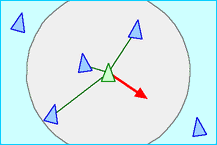
\includegraphics[width=0.45\textwidth]{img/separationdiagram.png}
            \label{fig:boidsep}
        }
        \subfigure[Angleichungs-Regel]{
            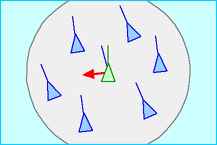
\includegraphics[width=0.45\textwidth]{img/alignmentdiagram.png}
            \label{fig:boidalign}        
        }
        \caption[Relevante Regeln der Boids]{Relevante Regeln der Boids}
        \label{fig:boid-rules}
    \end{center}
\end{figure}

\section{Hardware}

In diesem Abschnitt wird der technische Aufbau des \boidbot (siehe \figref{fig:boidbot}) beschrieben. Grundgerüst des \boidbot bildet eine 100\,cm$^2$ große Acrylglasplatte, an der alle weiteren Komponenten angebracht sind.

Insgesamt sind innerhalb dieses Projekts zwei Robotter entstanden, \boidbot I und \boidbot II.

Als Controller dient ein \emph{Arduino Uno}\footnote{www.arduino.cc}, dass mit einem selbstentworfenem Controller-Shield zur Steuerung des Antriebs und der Sensorik ausgestattet wurde. Das gesamte System wird durch eine Batterie mit einer Spannung von zirka 9,6 V versorgt. In \figref{fig:boidbot} sind die entwickelten Roboter abgebildet.

\fig{img/boidbota2r.jpg}{fig:boidbot}{\boidbot}{}

\subsection{Antrieb}

Auf der Unterseite der Grundplatte sind zwei Servomotoren angebracht, die den \boidbot antreiben sowie ein Stützrad. Die hier verbauten Servomotoren haben in ihrer ursprünglichen Bauform nur einen Einstellbereich von $270^\circ$ und somit als Antriebsmotoren nicht nutzbar. Daher wurden diese Motoren entsprechend modifiziert\footnote{http://www.fpoppa.de/brecker/robotik/tutorials/servo-mod}, damit sie als Antriebsmotoren einsetzbar sind.

Zum Antrieb des Sensor-Auslegers, der sich um den Roboter bewegt, ist auf der Grundplatte ein bipolarer Schrittmotor angebracht. Dieser bewegt den Ausleger Kreis um den \boidbot herum. So ist gewährleistet, dass möglichst wenig Sensoren benötigt werden, um den Bereich um den Roboter sensorisch abzudecken.

\subsection{Sensoren}

Am bereits erwähnten Sensorturm sind verschiedene Sensoren zur Abstandsmessung sowie zum senden und empfangen von Infrarotlicht angebracht. Die Abstandsmessung wird mit einem Infrarot-Proximity-Sensor vorgenommen, der am Ende des Sensor-Auslegers angebracht ist. Zum Senden von Infrarotlicht, sind drei Infrarot-LEDs über der Schrittmotorachse angebracht. Sie dienen dazu, den Roboter einem anderen \boidbot gegenüber identifizierbar zu machen. Um selber einen \boidbot zu erkennen, besitzt der Roboter einen Infrarotempfänger, der ebenfalls über der Schrittmotorachse in Richtung des Auslegerarms angebracht ist.

\subsection{Hardware-Controller}

Wie bereits erwähnt ist ein \emph{Arduino Uno} Basis der Hardwaresteuerung. Zusätzlich ist daran ein selbstentworfenes Controller-Shield angeschlossen, welches eine Schnittstelle zu den restlichen Komponenten des Systems bildet. Daran sind Stromversorgung, Schrittmotor, Sensoren und die Antriebs-Servo\-motoren angeschlossen. Für die Ansteuerung des Schrittmotors befindet sich auf dem Controllerboard ein \emph{L293D H-Driver}\footnote{http://www.datasheetcatalog.org/datasheet/texasinstruments/l293.pdf}. Die Servomotoren werden durch das Arduino gesteuert, allerdings mussten wir feststellen, dass durch den Umbau es keinen Ruhepunkt gibt, an denen die Motoren still stehen. Dies ist aber notwendig um den Roboter anzuhalten. Durch einen vorgeschalteten Transistor, kann für das Anhalten die Versorgungsspannung für die Servomotoren komplett abgeschaltet werden. In \figref{fig:schaltung} ist die Verschaltung der einzelnen Komponenten dargestellt.

\fig{img/schaltung.png}{fig:schaltung}{Schaltbild des Hardware-Controllers}{}

\section{Controller}

In diesem Abschnitt wird die entwickelte Software für die Roboter beschrieben. Die Grundplattform ist Arduino, daher wurde zur Erstellung der Software die Arduino Entwicklungsumgebung genutzt. Als Programmiersprache wird ein C-Dialekt verwendet.

\subsection{Verwendete Softwarekomponenten}

Die Arduino Plattform besitzt eine große Gemeinschaft, welche für viele Bauteile spezielle Bibliotheken zur Verfügung stellt. Diese erleichtern das Entwickeln von eigenen Projekten.

Es wurden Bibliothken für die Ansteuerung von Servos\footnote{http://www.arduino.cc/playground/ComponentLib/Servo}, einem Schrittmotor\footnote{http://arduino.cc/en/Reference/Stepper} und zur Steuerung der Infrarot LEDs\footnote{https://github.com/shirriff/Arduino-IRremote} genutzt.

\subsection{Grundverhalten}

Um den Sensorkopf, an dem der Distanzsensor und der Infrarotempfänger installiert sind, zu steuern wurde ein Schrittmotor genutzt. Dieser kann eine vollständige Umdrehung in 200 Schritten absolvieren. Das bedeutet, das ein Schritt dieses Motors den Schwenkkopf um 1{,}8$^\circ$ dreht.

Im Grundverhalten wird dieser Kopf im Halbkreis um den Roboter bewegt, damit er den kompletten Bereich vor ihm abtasten kann. In jedem Schritt wird die aktuell ermittelt Wert des Distanzmessers gelesen und verarbeitet.

Der Distanzsensor hat eine Reichweite von 10 bis 80 cm. Versorgt wird der Sensor über einen 5 V Anschluss. Je nach ermittelter Entfernung kann am Sensorausgang eine entsprechende Spannung abgelesen werden. Das Ablesen erfolgt mittels analogem Eingang am Arduino, welches die Eingangsspannung auf einen Wert zwischen 0 und 1023 abbildet.

Damit der jeweilige Roboter vom anderen erkannt werden kann, wird ein Infrarot Signal permanent ausgesendet. Dazu wird die IRremote Bibliothek genutzt, die es erlaubt beliebige Daten über Infrarot zu verschicken. Erkannt werden diese Lichtsignale über einen Infrarotempfänger. Dieser besitzt neben der Stromversorgung auch einen Signalausgang. Wird kein IR Signal empfangen, liegt an diesem 5 V an. Wird ein IR Signal erkannt, fällt die Spannung kurzfristig auf 0 V. Um diese Veränderung zu erkennen, wurde der Empfänger an einen Interrupt fähigen Pin des Arduinos angeschlossen. Kommt es zum Spannungsabfall an diesem Pin wird eine Funktion der Mikocontrollers aufgerufen. Dieser speichert zur weiteren Verarbeitung den aktuellen Winkel des Schwenkkopfes.

\subsection{Verhaltensbasierter Roboter}

Der Algorithmus basiert auf der Verwendung von verschiedenen Verhalten. Diese sind auf dem Roboter mittels einer Statusmaschine implementiert. Das Standardverhalten eines jeden Roboters ist es, gerade aus zu fahren. Falls ein Hindernis mittels des Schwenkarms entdeckt wurde, wird in den Status Objekt ausweichen gewechselt. Konnte mittels Infrarot Empfänger ein anderer Roboter erkannt werden, wird das Verhalten Roboter folgen genutzt.

\subsection{Algorithmus}

Programmiert man ein Arduino müssen mindestens zwei Funktionen implementiert werden. Zum einen eine setup Methode um sämtliche Sensoren zu initialisieren, zum anderen eine loop Funktion. Diese wird vom Mikrocontroller permanent aufgerufen. In dieser Funktion muss daher die Logik programmiert werden. Der Grundsätzliche Ablauf dieser Loop-Funktion ist in Algorithmus \ref{alg:roboter} skizziert.

Der Grundaufbau ist, das die Sensordaten ausgelesen werden und basierend darauf ein neuer Status gewählt wird. Könnte zum Beispiel ein Hindernis auf der linken Seite des Roboters erkannt werden, soll der Roboter nach rechts ausweichen. In den Stati Ausweichen und Folgen wird der Sensorkopf nicht bewegt. Der Grund ist, das so lange das Hindernis beobachtet werden soll bis er außerhalb des Gefahrenbereichs ist.

\begin{algorithm}
\caption{Programmablauf eines Roboters}
\label{alg:roboter}
\begin{algorithmic}
\STATE $sendIrSignal$
\IF{$s = FORWARD$}
    \STATE $moveSensorTurret$
    \STATE $readSensorData$
    \STATE $changeStateIfNessesary$
    \STATE $reactOnStateAndSensorData$
\ELSIF{$s = AVOID \lor s = FOLLOW$}
    \STATE $readSensorData$
    \STATE $changeStateIfNessesary$
    \STATE $reactOnStateAndSensorData$
\ENDIF
\end{algorithmic}
\end{algorithm}

\subsection{Probleme}

Auf dem Sensorturm sind drei Infrarot LEDs installiert. Zusätzlich wird zum erkennen des anderen Roboters ein Infrarot Sensor benutzt, der sich zusammen mit dem Turm dreht.

In Tests musste festgestellt werden, dass die Erkennung des Infrarot Lichts nur auf relativ geringe Distanzen funktioniert. Ein Grund dafür kann zum einen eine zu schwache Infrarot LED sein, zum anderen hat sich sie Ausrichtung der LED als weiteres Hindernis herausgestellt.

Wird der Sensorturm des anderen Roboters nicht bewegt, konnte über Distanzen von ca. 30 - 40 cm eine gute Erkennungsrate beim zweiten Roboter erzielt werden. Jedoch sollen beide Roboter durch einen Raum fahren können, dies erfordert das drehen des Sensorturms. In diesem Szenario war die Erkennungsrate sehr gering, eine akzeptable Leistung konnte nicht erzielt werden.

Zur Verbesserung der Erkennungsrate wird zum einen Vorgeschlagen stärkere Infrarot LEDs zu benutzen und zum anderen mehr von diesen auf dem Turm zu installieren. Damit wird erreicht, das in alle Richtungen das Signal ausgesandt und daher auch aus jeglichen Richtungen erkannt werden kann.

\section{Zusammenfassung}



%%%%%%%%%%%%%%%%%%%%%%%%%%%%
% Literaturverzeichnis
%%%%%%%%%%%%%%%%%%%%%%%%%%%%

%\newpage
%\nocite{*}
%\bibliography{books}
%\bibliographystyle{alphadin}

%%%%%%%%%%%%%%%%%%%%%%%%%%%%
% Anhang
%%%%%%%%%%%%%%%%%%%%%%%%%%%%

%\newpage
%\addcontentsline{toc}{section}{Anhang}

%\begin{appendix}

%\end{appendix}

\end{document}
